\chapter{Fundamentos tecnológicos}
En este capítulo, hablaremos sobre las herramientas escogidas para llevar a cabo el proyecto y el motivo por el que fueron seleccionadas.
En primer lugar comentaremos los servicios de \textit{Backend}, a continuación el servidor de localización en interiores y después las herramientas empleadas durante el desarrollo, especialmente de la aplicación \textit{iOS}. Finalizaremos con las herramientas de gestión del proyecto y de la documentación.

\section{\textit{Backend}}
En esta sección hablaremos del motivo por el que se optó por los servicios ofrecidos por \textit{Firebase}.

\subsection{Estudio alternativas y selección} 
\textit{Firebase} \cite{google_firebase_nodate} es una plataforma de \textit{Google} que nos ofrece una gran cantidad de servicios para desarrollar aplicaciones móviles, de los cuales hemos utilizado el servicio de autenticación, el de base de datos \textit{online} en tiempo real, el de ejecución de código propio y el de \textit{API REST}.

Se decidió utilizar \textit{Firebase} en lugar de crear un servicio propio, por la comodidad que ofrece esta plataforma al tener todos los servicios necesarios (figura~\ref{fig:firebase-services}), siendo el objetivo del proyecto una aplicación móvil y no un servidor web.

\begin{figure}[tbp]
\begin{center}
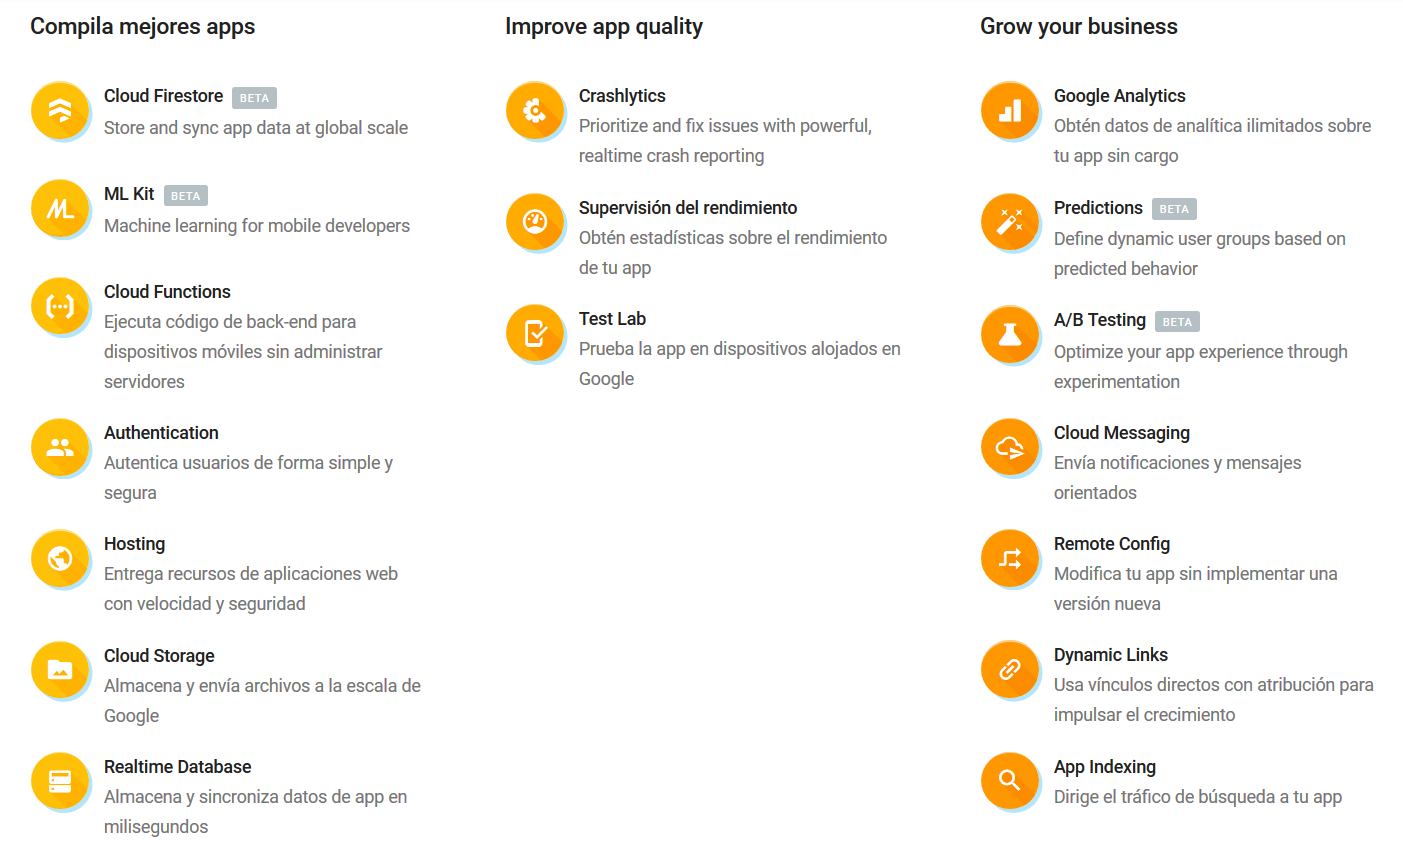
\includegraphics[scale=0.5]{figures/firebase.png}
\caption{Listado de servicios ofrecidos por \textit{Firebase}.\label{fig:firebase-services}}
\end{center}
\end{figure}

\subsection{Autenticación}
\textit{Firebase Authentication} \cite{google_firebase_nodate-1} busca facilitar la creación de sistemas de autenticación seguros, a la vez que mejora la experiencia de incorporación y acceso para los usuarios finales. Proporciona una solución de identidad de extremo a extremo, compatible con cuentas de correo electrónico y contraseñas, autenticación telefónica, \textit{Google}, \textit{Twitter}, \textit{Facebook}, acceso a través de \textit{GitHub} y más (ver subfigura~\ref{fig:auth_methods}).

Hay una gran cantidad de tutoriales \cite{firebase_tutorial_2016} para incorporar este sistema de autenticación a una aplicación \textit{iOS}, incluso hay vídeos oficiales de \textit{Google}. Aunque permite autenticarse de muchas maneras, en este proyecto sólo se contempla la autenticación mediante cuenta de \textit{Google}, no se consideró importante emplear tiempo en añadir otros métodos de inicio de sesión.

\subsection{Base de datos online en tiempo real}
Este servicio de \textit{Firebase} \cite{google_firebase_nodate-2} es uno de los más completos, ofreciendo un gran número de funcionalidades.
\paragraph{Sincronización en tiempo real para datos \textit{JSON}.} \textit{Firebase Realtime Database} es una base de datos \textit{NoSQL} alojada en la nube que te permite almacenar y sincronizar datos entre tus usuarios en tiempo real. Si accedemos a la consola de \textit{Firebase}, que es una página web desde la cual el administrador puede gestionar todos los servicios que tenga en su cuenta. Podemos ver la estructura de la base de datos (ver subfigura~\ref{fig:json}) y exportarla a un fichero \textit{JSON} o importarla de un fichero \textit{JSON}. Esto permite modificar la base de datos a nuestro gusto con un simple editor de texto.

\begin{figure}[tbp]
\begin{center}
\subfigure{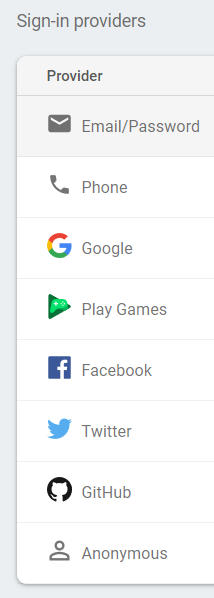
\includegraphics[height=9cm]{figures/fire_auth.png} \label{fig:auth_methods}}
\hspace{10ex}
\subfigure{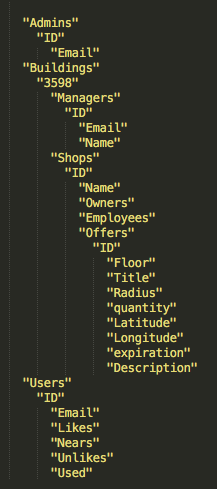
\includegraphics[height=9cm]{figures/json.png} \label{fig:json}}
\caption{\textit{Firebase}: (a) Métodos de autenticación permitidos y (b) almacenamiento de datos.}
\end{center}
\end{figure}

\paragraph{Colabora entre dispositivos con facilidad.} La sincronización en tiempo real permite que los usuarios accedan a sus datos desde cualquier dispositivo, web o móvil, y los ayuda a trabajar en conjunto.

\paragraph{Crea apps sin servidores.} \textit{Realtime Database} se incluye en los \textit{SDK} para dispositivos móviles y web, de manera que puedas crear apps sin la necesidad de usar servidores. También puedes ejecutar un código de \textit{Backend} que responda a los eventos que se activan con tu base de datos a través de \textit{Cloud Functions} \cite{google_firebase_nodate-3} para \textit{Firebase}.

\paragraph{Optimizada para el uso sin conexión.} Cuando los usuarios se desconectan, los \textit{SDK} de \textit{Realtime Database} usan la caché local del dispositivo para publicar y almacenar cambios. Cuando el dispositivo se conecta, los datos locales se sincronizan de manera automática.

\paragraph{Seguridad sólida basada en usuarios.} \textit{Realtime Database} se integra con \textit{Firebase Authentication} para brindar autenticación intuitiva y sencilla para los programadores. Se puede usar su modelo de seguridad declarativo para permitir el acceso según la identidad de los usuarios o con patrones que coinciden con tus datos.

\subsection{Ejecución de código: \textit{Cloud Functions}\label{sec:cloud_functions}}
Determinadas tareas serían imposibles de realizar únicamente mediante peticiones a la base de datos desde el cliente. Por ello, \textit{Firebase} ofrece la posibilidad de subir a su plataforma no sólo datos, sino también funciones \cite{noauthor_cloud_nodate}. Esta es una de las últimas funcionalidades que se han añadido a \textit{Firebase} y todavía se encuentra en estado beta, pero ya se dispone de una gran comunidad de usuarios que la utiliza, así como mucha información en Internet, guías de uso y ejemplos \cite{noauthor_cloud_nodate-1}.

El lenguaje que se utiliza es \textit{JavaScript} aunque también se nos da la posibilidad de escribir nuestras funciones en \textit{TypeScript}. Además disponemos de una amplia documentación para iniciarnos en el desarrollo de \textit{Cloud Functions}, como es habitual en todos los productos que ofrece \textit{Firebase} \cite{noauthor_documentacion_nodate}. Hay varios tipos de funciones que se pueden subir a la plataforma para interactuar con nuestra base de datos, pero sólo hemos utilizado dos: activadas por una petición HTTP o por un cambio en la base de datos.

\paragraph{Funciones activadas por una petición \textit{HTTP}.} Cada una de ellas tiene asociada una \textit{URL}, a la cual debemos realizar una petición cualquiera (\textit{GET}, \textit{HEAD}, \textit{POST}, etc.) si queremos que se ejecute. Desde estas funciones podemos leer y modificar nodos de la base de datos. Son muy útiles si lo que queremos es realizar acciones periódicas en la base de datos, en nuestro caso, recorrer la base de datos para eliminar aquellas ofertas que hayan caducado \cite{noauthor_http_nodate}.

\paragraph{Funciones activadas por un cambio en la base de datos.} Estas funciones no se pueden activar mediante una petición \textit{HTTP} como las anteriores, en este caso, será una modificación de la base de datos la que provocará que se ejecuten. En lugar de asociarles una \textit{URL}, lo que debemos hacer es asociar cada función a un nodo de la base de datos e indicarle ante que cambio en el mismo deberá ejecutarse \cite{noauthor_realtime_nodate}.

\begin{itemize}
\item[-] \textbf{\textit{onWrite}.} Tras la modificación, creación o eliminación de un dato.
\item[-]\textbf{\textit{onChange}.} Tras la modificación de un dato.
\item[-]\textbf{\textit{onDelete}.} Tras la eliminación de un dato.
\item[-]\textbf{\textit{onCreate}.} Tras la creación de un nuevo dato.
\end{itemize}

En este proyecto, se utilizan estas funciones para eliminar una oferta cuando se han agotado las existencias: cada vez que alguien la canjea, se escribe este escaneo en la oferta, lo cual es detectado por la función que resta uno al número de ofertas disponibles y si llega a cero, la borra de la base de datos.


\subsubsection{Otras consideraciones sobre las \textit{Cloud Functions}}
Un inconveniente de esta herramienta, es que cada vez que se realiza un cambio en una función hay que subirla de nuevo a \textit{Firebase} para ver si esto funciona. Cada una de estas operaciones puede llegar a tardar varios minutos, así que para usuarios no muy experimentados con \textit{Firebase} y \textit{JavaScript}, es recomendable crear un entorno local en el que probar que el código funciona antes de subirlo para no perder mucho tiempo \cite{noauthor_cloud_nodate}.
Además es difícil \textit{debuguear} estos programas, una opción es imprimir \textit{logs}, los cuales se mostrarán en la herramienta web de \textit{Cloud Functions} (subfigura~\ref{fig:logs}). 
También hay la posibilidad de mostrar las funciones que están corriendo en ese momento (subfigura~\ref{fig:functions}).
O de ver las estadísticas sobre las invocaciones que se han llevado a cabo (subfigura~\ref{fig:invocations}).

\begin{figure}[tbp]
\centering
\subfigure{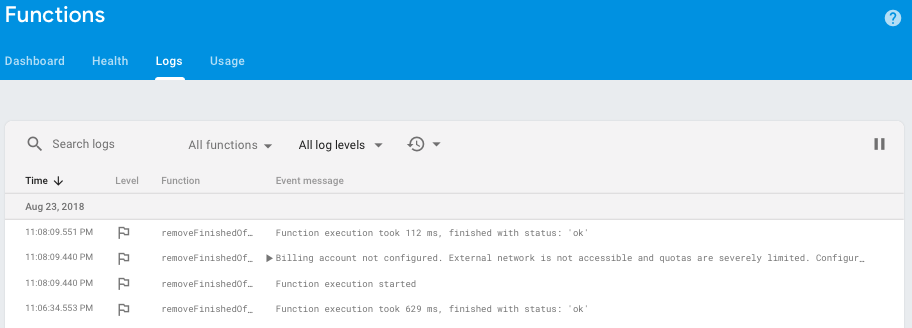
\includegraphics[width=0.9\textwidth]{figures/logs.png}\label{fig:logs}}
\subfigure{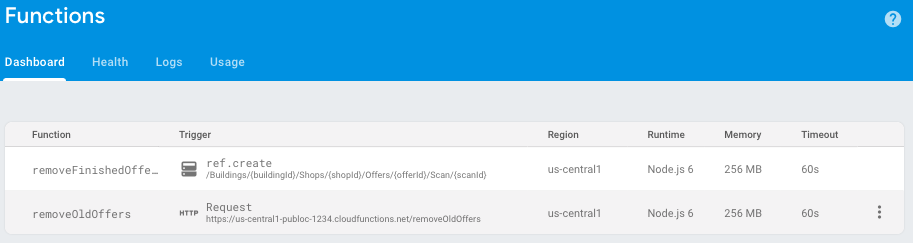
\includegraphics[width=0.9\textwidth]{figures/functions.png}\label{fig:functions}}
\subfigure{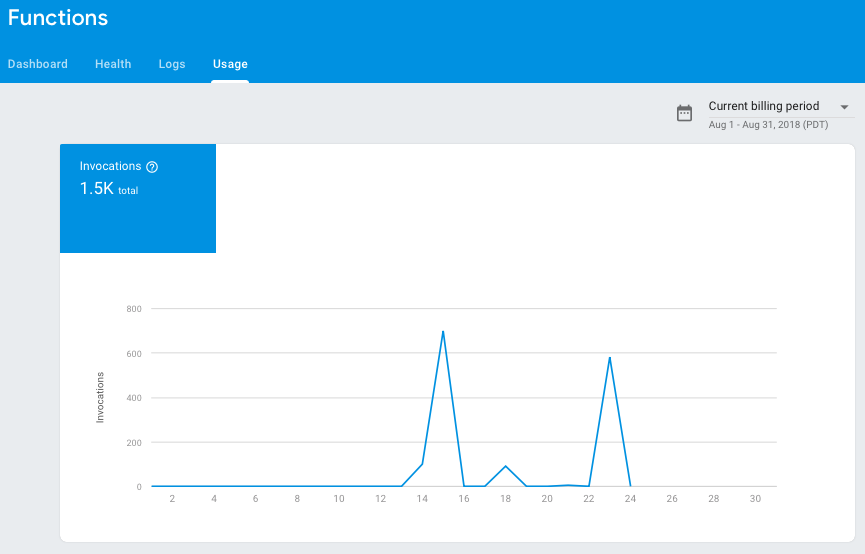
\includegraphics[width=0.9\textwidth]{figures/invocations.png}\label{fig:invocations}}
\caption{\textit{Cloud Functions console}: (a) \textit{Logs} de la ejecución de las diferentes funciones, (b) funciones en ejecución y (c) estadísticas sobre invocaciones de \textit{Cloud Functions}.}
\end{figure}

\subsubsection{Riesgos de las \textit{Cloud Functions}}
Una situación a evitar utilizando \textit{Cloud Functions}, es la recursividad. Una función que se lanza tras una escritura en un nodo de la base de datos puede escribir en ese mismo nodo, si esto sucede se producirá un bucle de escrituras que sólo parará si detenemos la ejecución de la función.

Si nos damos cuenta tarde corremos el riesgo de agotar el cupo de escrituras que nos ofrece \textit{Firebase} con el plan que tengamos contratado y si pagamos bajo demanda podemos llegar a perder bastante dinero si no descubrimos el fallo rápidamente.

\subsection{Comunicaciones en tiempo real: \textit{API REST}}
Se puede acceder a la base de datos desde el código directamente, gracias a las librerías de \textit{Firebase} que debemos importar en el proyecto. Tanto con \textit{Swift} \cite{firebase_firebasedatabase_2018} como con \textit{Objective-C} \cite{firebase_firebasedatabase_2018-1}. Pero en este proyecto se decidió utilizar el \textit{API REST}, debido a la extensa documentación \cite{firebase_firebase_2018} que podemos encontrar en la página oficial, además de que podemos probar las peticiones con más facilidad gracias a herramientas como \textit{Postman}.

\begin{figure}[tbp]
\begin{center}
\subfigure{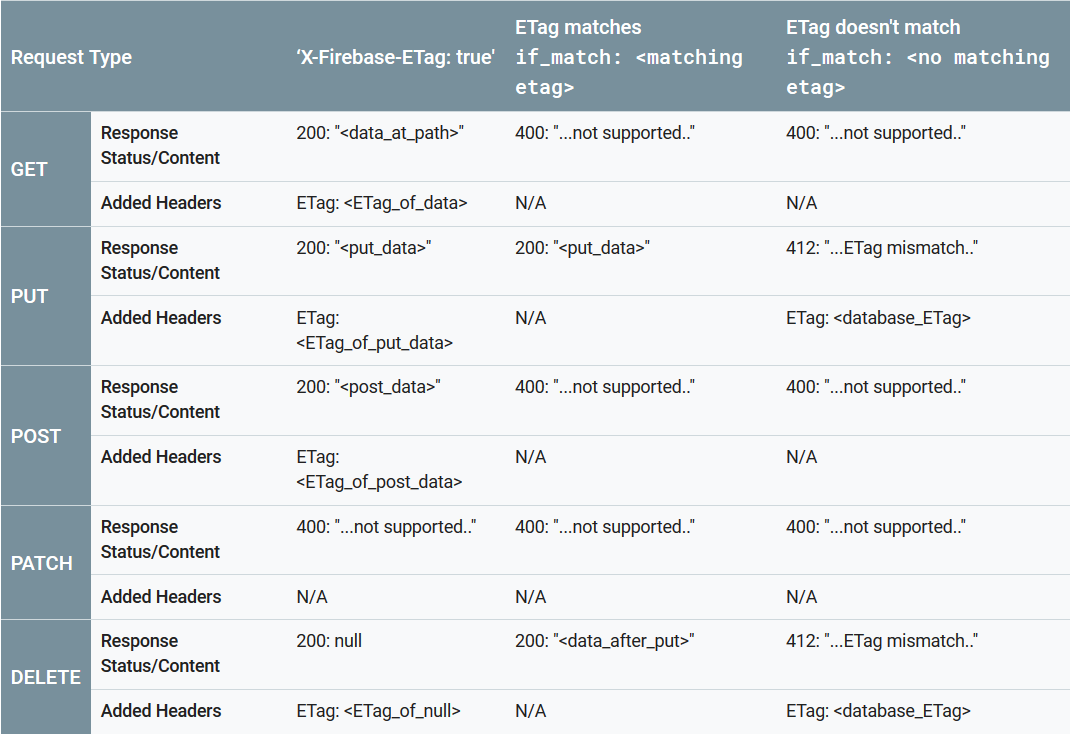
\includegraphics[width=0.9\textwidth]{figures/api_rest.png}}
\subfigure{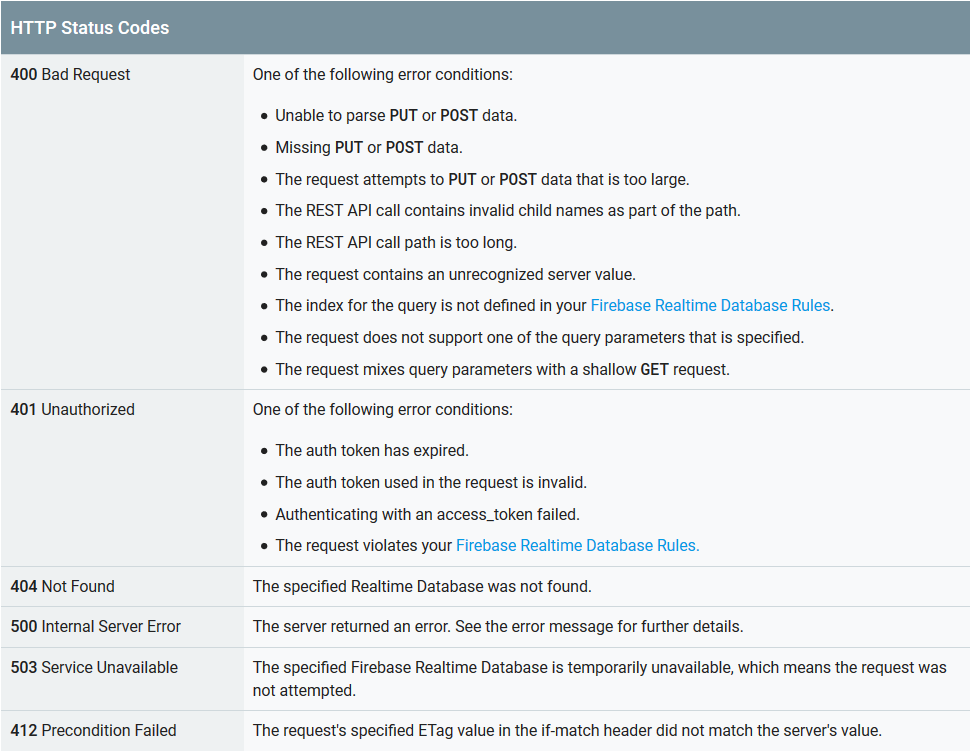
\includegraphics[width=0.9\textwidth]{figures/errors_rest.png}}
\caption{Peticiones \textit{API REST Firebase} y posibles código de errores.}
\end{center}
\end{figure}

Tiene peticiones básicas que permiten variaciones que las hacen más complejas: se puede añadir \textit{tokens} de autenticación en la \textit{URL}, se pueden descargar ficheros, obtener datos ordenados \cite{firebase_firebase_2018-1} o filtrados \cite{firebase_firebase_2018-2}, hacer \textit{streaming} de un valor de la base de datos para tener siempre su valor actualizado, etcétera.

\subsubsection{\textit{Streaming} mediante \textit{API REST}}
Para realizar \textit{streaming} de un nodo a través de la \textit{API REST}, lo que debemos hacer es enviar la cabecera \textit{\textbf{``Accept''}} de la petición con valor \textit{\textbf{``text/event-stream''}}. Esto es posible gracias a que \textit{Firebase} soporta el protocolo \textit{EventSource / Server-Sent Events} \cite{noauthor_eventsource_nodate}.

\section{Servidor localización en interiores \textit{Situm}}
El \textit{SDK} de \textit{Situm} nos da nuestra ubicación en espacios cerrados sin necesidad de añadir infraestructura. Al crearnos una cuenta en la plataforma, podemos empezar a subir mapas de nuestros edificios y calibrarlos.

\subsection{\textit{SDK}}
Es la librería que necesitamos para interactuar con la plataforma \textit{Situm} desde nuestra aplicación móvil. De esta manera, les transmitiremos la información recogida por los sensores de nuestro teléfono y nos será devuelta nuestra posición.

Esta librería también nos permite descargarnos los mapas y toda la información sobre los edificios. Actualmente, hay disponible \textit{SDK} para \textit{iOS} \cite{situm_situm_nodate}, \textit{Android} \cite{situm_situm_nodate-2} y \textit{Cordova} \cite{situm_situm_nodate-1}. Además de un \textit{API REST} \cite{situm_situm_nodate-3}.

\subsection{\textit{Dashboard}}
Mediante esta herramienta web, se pueden crear y editar edificios (subfigura~\ref{fig:mapa_situm_fic}), gestionar calibraciones, descargarnos sesiones de uso y más, ver subfigura~\ref{fig:funcionalidades_situm}.

\begin{figure}[t]
\centering
\subfigure{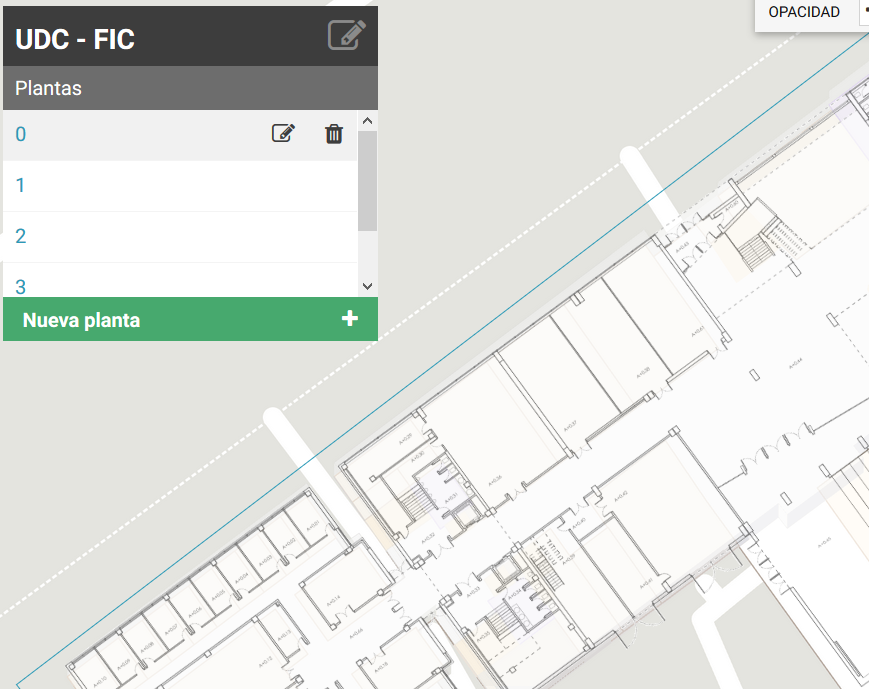
\includegraphics[width=0.4\textwidth]{figures/mapa_situm_fic.png}\label{fig:mapa_situm_fic}}
\subfigure{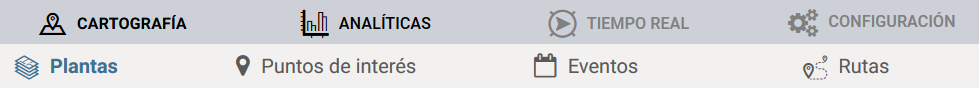
\includegraphics[scale=0.5]{figures/funcionalidades_situm.png}\label{fig:funcionalidades_situm}}
\caption{\textit{Situm Dashboard}: (a) Funcionalidad de añadir planos para las diferentes plantas de un edificio y (b) otras funcionalidades de \textit{Situm Dashboard}.}
\end{figure}

\subsection{\textit{Situm Mapping Tool}}
Es una aplicación para móviles \textit{Android} que nos permite acceder a la cuenta de \textit{Situm} para subir calibraciones al \textit{Dashboard}.

\subsubsection{Alternativas a \textit{Situm}}
Desde el comienzo del proyecto se impuso como requisito la utilización de esta plataforma, pero eso no quiere decir que sea la única que ofrece este tipo de servicios, un par de ejemplos:  \textit{IndoorAtlas} \cite{noauthor_indooratlas_nodate} y \textit{Senion} \cite{noauthor_senion_nodate}.


\section{Desarrollo aplicación \textit{iOS}}
En esta sección se comentaran aquellas tecnologías que fueron necesarias para la realización de este trabajo concreto, y también se hablará sobre las alternativas disponibles.

\subsection{\textit{Swift}}
El lenguaje de programación elegido fue \textit{Swift}. Otra alternativa sería utilizar \textit{Objective-C}, el antecesor de \textit{Swift}. Para aplicaciones antiguas que necesitan mantenimiento es interesante conocer \textit{Objective-C}, pero la tendencia actual es hacer todo en \textit{Swift}, ya que es un lenguaje mucho más intuitivo y está especialmente diseñado para desarrollar aplicaciones \textit{iOS}, ver figura~\ref{fig:objc_swift}.

\begin{figure}[tbp]
\centering
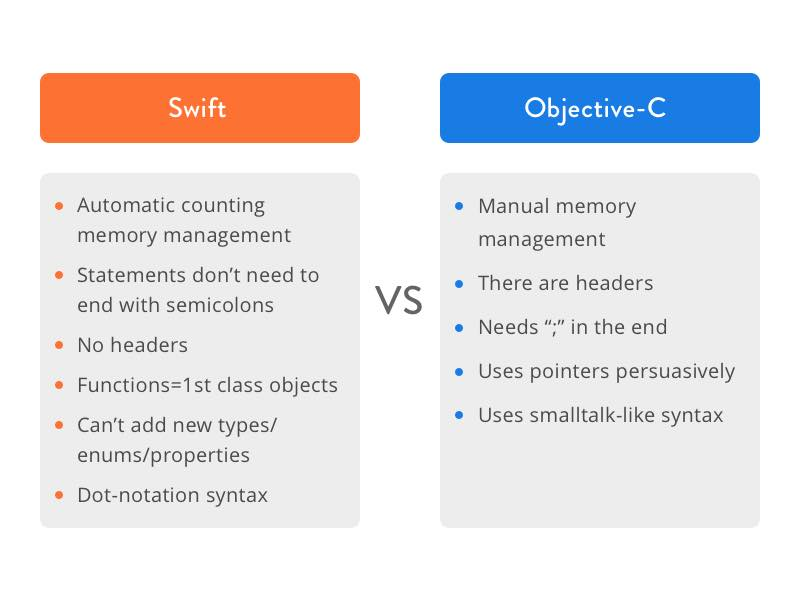
\includegraphics[scale=0.45]{figures/objc_swift.jpg}
\caption{Algunas diferencias entre los dos lenguajes.\label{fig:objc_swift}}
\end{figure}

\subsection{\textit{Alamofire}}
Esta librería \cite{noauthor_alamofire_nodate} fue incluida en el \textit{app iOS} para realizar todas las peticiones \textit{HTTP} necesarias, así como el \textit{streming} de nodos de la base de datos.

\subsection{\textit{Postman}}
Este programa que se puede descargar para \textit{Mac}, \textit{Windows} y \textit{Linux} \cite{noauthor_postman_nodate}. Tiene planes de pago pero para nootros con el gratuito fue suficiente.
Con esta herramienta podemos probar las peticiones antes de incorporarlas a la aplicación, ver que códigos de error se obtienen, etcétera.

\subsection{iOS}
La decisión de hacer una aplicación para \textit{iOS} en lugar de para \textit{Android} se debe a que ya se disponía de las herramientas necesarias (ordenador con sistema operativo \textit{macOS} y un \textit{iPhone}), y sobre todo, al tipo de aplicación que se va a desarrollar.

Los \textit{iPhones} son teléfonos caros y suelen estar en manos de personas con un poder adquisitivo más alto. Como prueba, a pesar de tener un menor número de usuarios que \textit{Android} a nivel mundial, el \textit{App Store} (la tienda de aplicaciones de \textit{Apple}) genera muchos más ingresos que el \textit{Play Store} (tienda de aplicaciones \textit{Android}) \cite{christian_collado_app_2018}. Al ser una aplicación con un propósito consumista, es lógico pensar que tendrá una mayor acogida entre los usuarios de \textit{iOS} que entre los de \textit{Android}.


\section{Tecnologías de edición y gestión}
En esta sección, hablaremos sobre las herramientas de edición utilizadas durante el proyecto:

\subsection{Xcode}
Para crear aplicaciones para \textit{iOS}, es necesario el programa \textit{Xcode}, si se dispone de un ordenador con sistema operativo \textit{macOS}, se puede obtener de manera gratuita. Pero muchas veces no se dispone de este \textit{Hardware}, en este caso hay alternativas \cite{chris_ching_xcode_2017} como instalar dicho sistema operativo en una máquina virtual, o bien alquilar una máquina en la nube.


\subsection{\textit{IconJar}}
Para descargar iconos en formato \textit{PDF}, necesarios para la aplicación, se utilizó el programa \textit{IconJar} \cite{curtis_hard_davey_heuser_iconjar_nodate} en su versión gratuita.
\begin{figure}[tbp]
\begin{center}
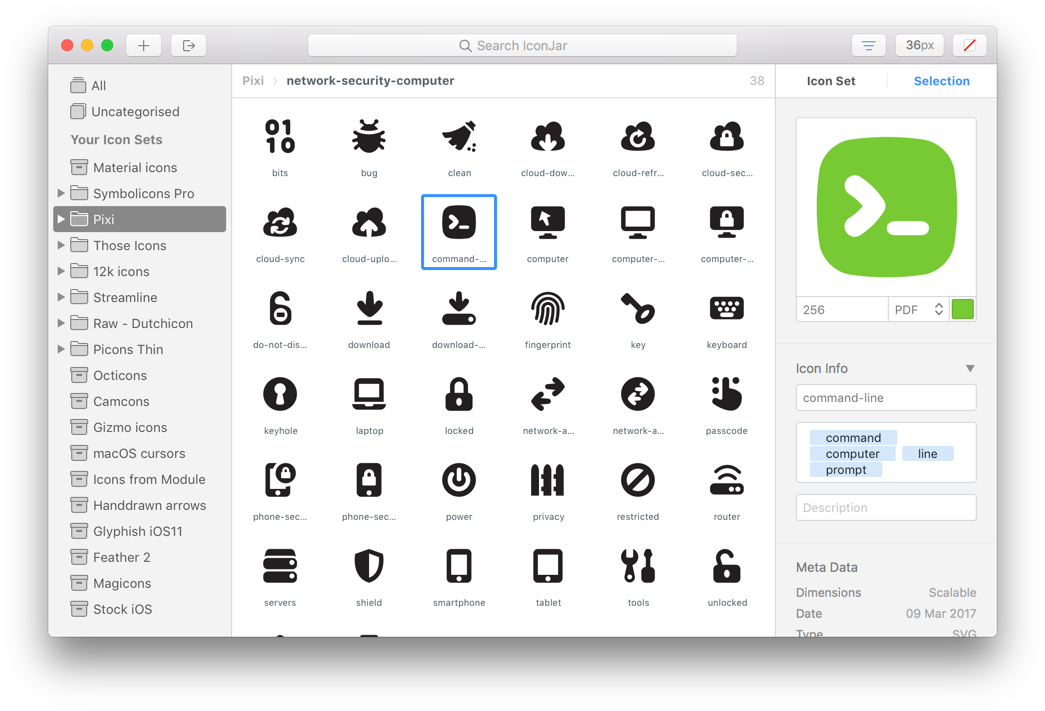
\includegraphics[scale=0.37]{figures/iconjar.png}
\caption{Generación de iconos con \textit{IconJar}.}
\end{center}
\end{figure}

\subsection{\textit{Adobe Xd}}
Para el diseño de pantallas e interfaces, se utilizó el programa \textit{Adobe Xd }\cite{noauthor_adobe_nodate}, también en su versión gratuita.
Para aprender a manejar esta herramienta es recomendable seguir tutoriales \cite{forrestknight_how_nodate}, sobre todo al principio.
Se deben utilizar este tipo de programas para realizar los diseños, porque si intentamos llevarlos a cabo sin planificar, lo que va a pasar es que tengamos que compilar el programa cada vez que realicemos un pequeño cambio. En cambio, si ya sabemos como queremos la \textit{app}, podemos programarlo todo y compilar al final sabiendo que va a quedar bien.

\subsection{\textit{Git}}
Para el control de versiones, se utilizó el \textit{Git} \cite{noauthor_git_nodate} de la facultad. En el cual todos los alumnos podemos entrar con nuestra cuenta y crear proyectos privados de manera gratuita.

\begin{figure}[tbp]
\centering
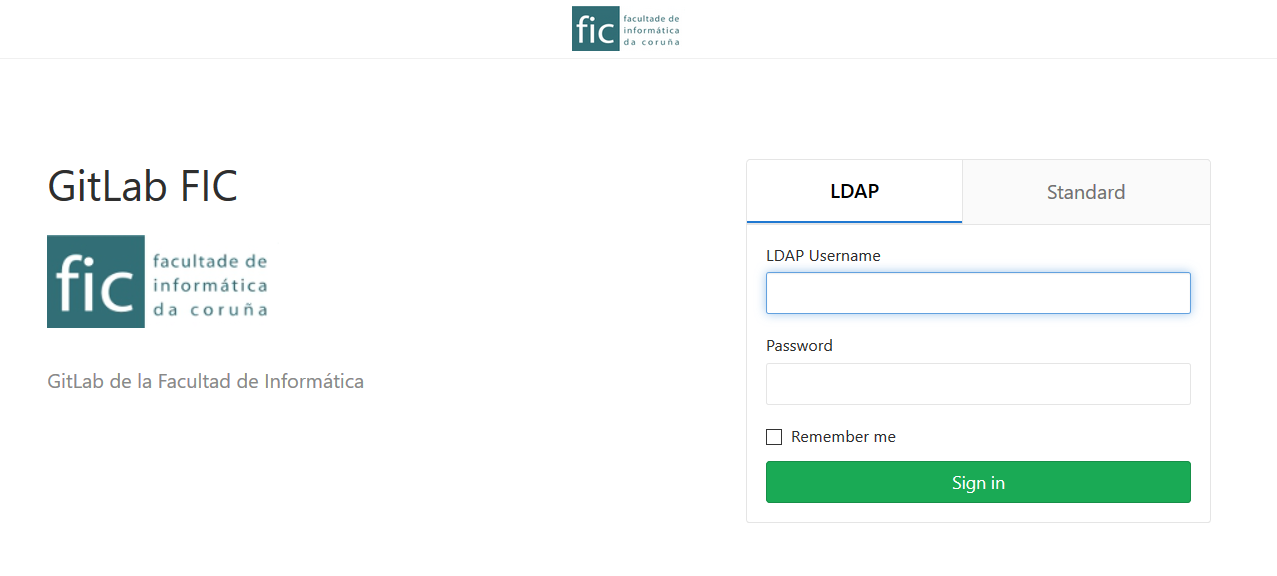
\includegraphics[scale=0.5]{figures/gitfic.png}
\caption{Se inicia sesión con la cuenta de la Universidad}
\end{figure}

\subsection{\textit{LaTeX}}
Para redactar la memoria, se escogió \textit{LaTeX} porque da unos resultados muy elegantes y la complicación es mínima.

Para facilitar la tarea se utilizó una herramienta web llamada \textit{Overleaf} \cite{noauthor_overleaf_nodate} en su versión gratuita. La cual permite compartir el documento con un \textit{link} para que varias personas puedan leerlo y/o editarlo. También lo sube a \textit{Git}, dándonos un enlace mediante el cual podemos clonarlo para guardar una copia en nuestro ordenador personal. Cabe destacar que esta herramienta ofrece la posibilidad de compilar a medida que escribimos, así podemos ver resultados casi inmediatamente.

\subsection{\textit{GanttProject}}
A la hora de elaborar un diagrama de \textit{Gantt} para planificar el desarrollo del proyecto, se optó por utilizar una herramienta de software libre llamada \textit{GanttProject} \cite{noauthor_ganttproject_nodate}. Es una herramienta que ofrece menos funcionalidades que otras como \textit{Microsoft Project}, pero mucho más fácil de usar.

Algunas de las funcionalidades que ofrece son: gráficos \textit{PERT}, creación de informes en formato \textit{PDF} y \textit{HTML}, importación y exportación de documentos en formato \textit{MS Project}, importación y exportación de datos contenidos en hojas de cálculo, creación de diagramas de \textit{Gantt}, jerarquías y dependencias entre tareas, etcétera.
No es la única herramienta de software libre para gestionar proyectos \cite{ruben_alcaraz_3_2012}, aquí podemos encontrar un breve tutorial para iniciarnos con esta herramienta \cite{dmitry_barashev_ganttproject_2011}.